% !TeX spellcheck = en_US

\documentclass[a4paper]{article}
\usepackage[utf8x]{inputenc}	% Use UTF8 characters
\usepackage[hyphens]{url}	% Proper url in the references section
\usepackage{relsize}		% Provide \mathlarger to get formula's to the correct size
\usepackage{hyperref}		% Clickable urls and references ("\pdfendlink ended up in different nesting level than \pdfstartlink"? add [draft])
\usepackage{enumitem}		% Numbered items, enumerate customizers
\usepackage{graphicx}		% Images
\usepackage{tabularx}		% Tables
\usepackage{needspace}		% Prevent sections starting when low on space
\usepackage{placeins}		% \FloatBarrier
\usepackage{longtable}		% Multi-page tables
\usepackage[nottoc,numbib]{tocbibind} % Add reference to the table of contents (and give it a chapter number)

\emergencystretch=10pt		% Allow more stretching whitespace to prevent overfull/underfilled lines.

% TODO: use \Needspace{5\baselineskip} before sections (redefine sections?)
\usepackage[usenames, dvipsnames]{color}
\usepackage[toc,page]{appendix}
\definecolor{inline}{rgb}{0,0,0.5}
\pagenumbering{arabic}		% Page numbering
\setlist{itemsep=0pt, topsep=2pt} % Smaller spacing between items
% \overlap for week numbers that are used twice
\definecolor{overlap}{gray}{0.5}
\newcommand{\overlap}[1]{\textcolor{overlap}{#1}}

\newcommand{\sectionbreak}{\clearpage} % Newpage before starting new section

% Setup section header spacing
\usepackage{titlesec}
\titlespacing*{\section}
	{0pt}{0.7cm}{0cm}
\titlespacing*{\subsection}
	{0pt}{0.7cm minus 0.4cm}{0cm}
\titlespacing*{\subsubsection}
	{0pt}{0.4cm minus 0.2cm}{0cm}

% Setup captions styling
\usepackage{caption}
\captionsetup[figure]{format=plain, singlelinecheck=false, margin=0pt, font={bf,footnotesize}, justification=centering, aboveskip=3pt}
\captionsetup[table]{format=plain, singlelinecheck=false, margin=0pt, font={bf,footnotesize}, justification=centering, aboveskip=3pt}
\captionsetup[lstlisting]{format=plain, singlelinecheck=false, margin=0pt, font={bf,footnotesize}, justification=centering, aboveskip=3pt}

% Setup todo note command
\marginparsep 11pt
\marginparwidth 1.4cm
\usepackage{setspace}	% \setstretch
\newcommand{\todo}[1]{{\color{BurntOrange}\sffamily\textbf{todo: #1}\par}}

\setlength{\parindent}{0em} % No indenting for new paragraphs
\setlength{\parskip}{0.5em} % Empty line between paragraphs

% Spacing of tableofcontents
\usepackage{tocloft}
\renewcommand\cftsecafterpnum{\vskip0pt}

% Code listings
%===== Code snippet styling =====
\newcommand{\code}[1]{\texttt{\small \color{inline}#1}} % \code command for inline snippets
\usepackage{listings}		% Code snippets
\usepackage{color}			% Code highlighting colors
\definecolor{dkgreen}{rgb}{0,0.6,0}
\definecolor{inline}{rgb}{0,0,0.5}
\definecolor{gray}{gray}{0.2}
\definecolor{codeText}{rgb}{0.1,0.1,0.1}
\definecolor{mauve}{rgb}{0.58,0,0.82}
\lstset{frame=tb,
	framerule=0.2pt,
	language=Java,
	aboveskip=2mm,
	belowskip=5mm,
	showstringspaces=false,
	columns=flexible,
	basicstyle={\small\ttfamily\color{codeText}},
	numbers=left,
	numbersep=4pt,
	numberstyle=\tiny\color{gray},
	keywordstyle=\color{blue},
	commentstyle=\color{dkgreen},
	stringstyle=\color{mauve},
	breaklines=true,
	breakatwhitespace=true,
	tabsize=4
}
\lstdefinelanguage{YAML}
{%
	alsoother     = @\$,
	morecomment   = **[l]{\#},
	morecomment   = **[s]{/*}{*/},
	morestring    = **[s]{"}{"},
}[keywords,strings,comments]
\lstset{language=YAML} % Set default language

\lstdefinelanguage{JSON}
{%
	string       = [s]{"}{"},
	stringstyle  = \color{blue},
	comment      = [l]{:},
	commentstyle = \color{black},
}[strings,comments]

\begin{document}

\begin{titlepage}
	\begin{center}
		{\huge\bfseries Verification of the Prefix Sum Program in an OpenCL Environment\par}
		
		\vspace{1cm}
		{\LARGE Thijs Wiefferink\par}
		{\large thijs@wiefferink.me, s1366564}
		
		\vfill
		
		{\Large
			University of Twente		
		}
	\end{center}

\end{titlepage}
\newpage


\section*{Abstract}
\todo{write}


\section*{Keywords}
\todo{write}


\section*{Preface}
This project is the continuation of my bachelor thesis project, in which the verification of the prefix sum algorithm has been started. Since only the 'data race free' part has been proven for the first part of the algorithm (the upsweep), the goal of this project is to prove the complete algorithm data race free, and additionally prove the functionality of the algorithm.

The necessary background information will be included in this report to understand the goal and results of the project, but full details of the Bachelor project can be read in the paper of that project \cite{bachelorThesis}.


\newpage
\tableofcontents


\section{Introduction}
This chapter describes the research domain, shows the problem that is solved, introduces the research questions and explains the approach.

\subsection{Research domain}
In this section the context information of this research project is described.

\subsubsection{GPU computing}
A graphics processing unit (GPU) is a device designed to rapidly manipulate and alter memory to accelerate the creation of images, for example while watching a video or playing a game. However, GPUs are also used more for general purpose computing, which is traditionally handled by the central processing unit (CPU). GPUs are better than CPUs doing parallel execution on large data sets. For example increasing the brightness of an image is easily done by a GPU, since this operation can be done in parallel on all pixels of the image. GPUs are however also used for physics calculations or mining crypto currencies. When using a GPU for general computing an API has to be used, I have chosen OpenCL for the previous research project because of its hardware vendor independency and open source nature. 

Running a parallel computation on a GPU brings a couple of challenges. The first challenge is preventing data races. A data race is the situation in a program where multiple threads are accessing the same memory location, with at least one of them writing to the location. The second challenge is verifying the correctness of the functionality of the program. Verifying both of these aspects is useful for safety critical systems.

The previous research project has started with the verification process to show that a program (specifically the Prefix Sum algorithm) has no data races. Since only the first half of the program could be verified in the given time for the project the verification has been continued in this project.

\subsubsection{Prefix Sum}
To show what the prefix sum is and how it is calculated, this section repeats the information from the previous project\cite{bachelorThesis} below.

The algorithm computes the sums of all possible prefixes of an input array. In Figure~\ref{prefixsumexample}, a mathematical representation of the prefix sum is illustrated, $x$ represents the input array, $x_0$ indicates the first element from the input array, where $n$ represents the size of the input array, and $y$ is the output array containing the prefix sums. Each number $y_a$ in the output array is the sum of all numbers $x_b \in x$ for which the condition $b<a$ holds.

\begin{figure}[htb!]
	\centering
	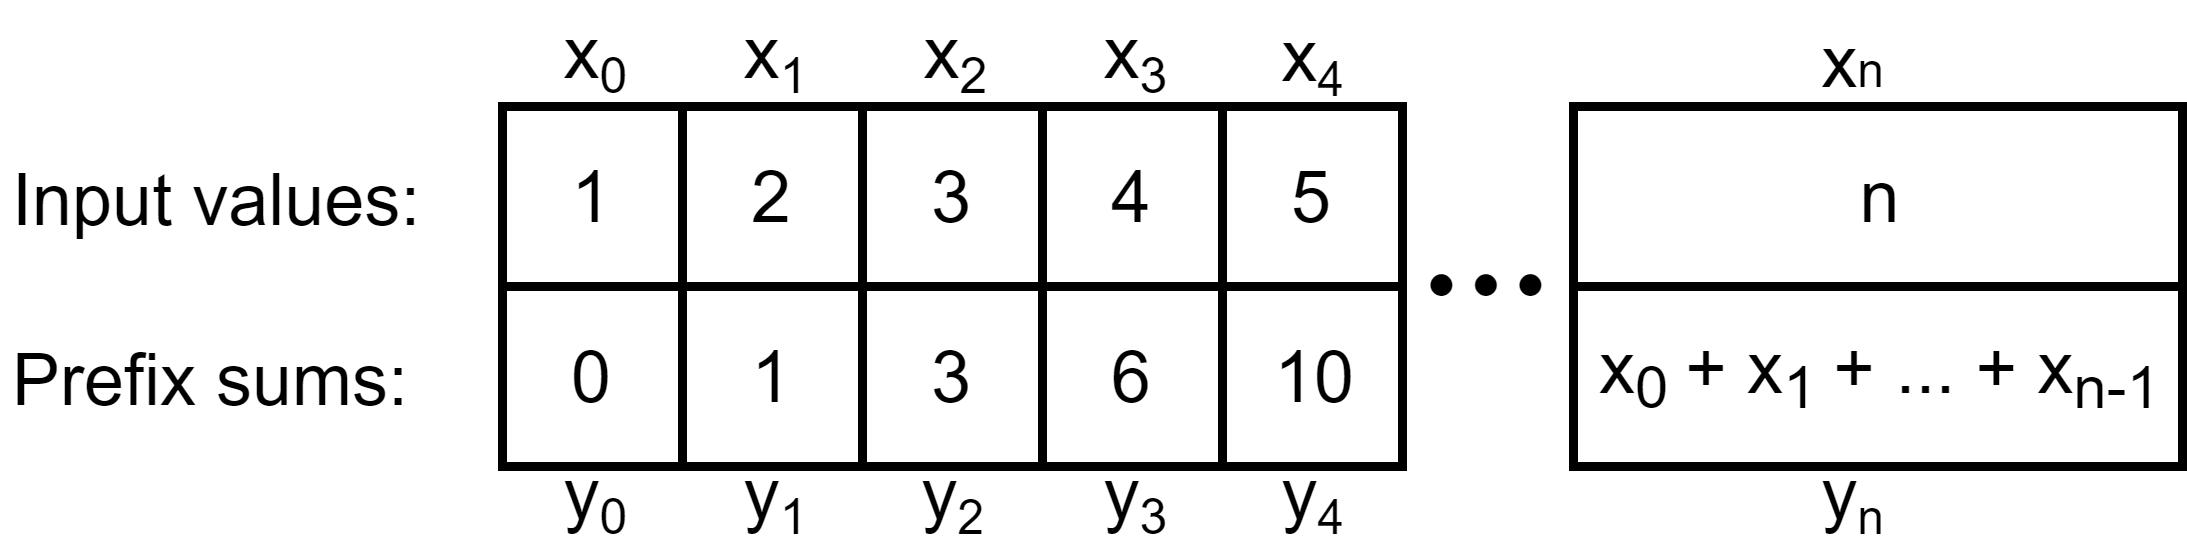
\includegraphics[width=80mm]{../images/prefix-sum-v1.png}
	\caption{Prefix Sum description}
	\label{prefixsumexample}
\end{figure}

The Prefix Sum algorithm is an interesting case study because it is a building block for a lot of other algorithms. For example radix sort and quicksort can be implemented using Prefix Sums, but it can also be used to lexically compare strings of characters or to search for regular expressions \cite{Blelloch:PrefixSumApplications}. In the field of specifying and verifying GPU programs the Prefix Sum is a suitable next step, because it will be a bigger and more complex example of verifying a GPU program.

The algorithm to calculate prefix sums can be structured in such a way that large amounts of data can be processed in parallel. A multi threaded algorithm meant for the GPU has been implemented in the previous project. The verification process continues with this same algorithm. The implemented version of the Prefix Sum is based on Chapter 39 \emph{Parallel Prefix Sum (Scan) with CUDA} of the book GPU Gems 3 \cite{Nguyen:GPUGems3}.

\subsubsection{Verification}
For the verification of the Prefix Sum program Permission-Based Separation Logic is used to specify the behavior of the program, and the tool VerCors is used to verify that the code matches the specification. A description of Permission-Based Separation Logic can be found in the previous project\cite{bachelorThesis}. 

\subsection{Problem statement}
\todo{use of verification}

\subsection{Research question}
\todo{write}

\subsection{Approach}
\todo{verification process and problem solving}

\subsection{Report structure}
\todo{introduce chapters}


\section{Prefix sum algorithm}
\todo{explain parallel prefix sum, based on bachelorreferaat paper}


\section{Verifying permissions}
\todo{verification process of the read/write permissions of the array (initial based on bachelorreferaat, extended to allow functional verification)}


\section{Verifying functionality}
\todo{verification process of the functionality of the program}


\section{Discussion}
\todo{summary}

\subsection{Results}
\todo{result description: verified}

\subsection{Related work}
\todo{similar verification projects}


\section{Conclusion}
\todo{summary}

\subsection{Research question answer}
\todo{works, not for huge programs though}

\subsection{Limitations and problems}
\todo{tool limitations, change code for verification process}

\subsection{Research value}
\todo{do larger programs, improve tool, concurrency}

\subsection{Future work}
\todo{larger programs, improve tool}


\bibliographystyle{abbrv}
\bibliography{Report}

\end{document}
